% !TEX root = ../thesis_main.tex
\chapter{Results}\label{chap:results}
    As a large part of this work consisted of hardware design and manufacturing, I will split the results section into sole hardware results and results of measurements \textit{with} that hardware as well as commercially available machines. Additionally, simulation results will be added as a separate section in the end of this chapter.
\section{Hardware}
    This section will cover the results concerning the hardware built in the course of this thesis. This covers calibration results as well as performance measurements of single components. If results were acquired by the workshop, this will be clearly indicated.
    \subsection{Low field NMR}
        The setup used mostly in the beginnning of the thesis work was the low field spectrometer. It needed to be calibrated and shimmed and experiments with various substances and in various settings were performed.
        \subsubsection{Receive coils}
        Receive circuits provided a Q-factor of 128 as shown in figure \ref{fig:results:networkAnalysis}.  An additional, higher frequency resonance with Q-factor of 32 can be seen to the right in the same plot at around \SI{460}{\kilo Hz}. The second graph shows the same measurement performed with the untuned saddle coil. The latter shows no significant dips and is thus considered broadband, i.e. as long as the RF-amplifiers power is sufficient, it can be used at arbitrary frequencies. Note that additional impedances are introduced into the system through the connection to the NI DAQ interface that cannot be neglected especially in the higher frequency range above $\SI{100}{\kilo\hertz}$ where the coil's intrinsic capacities are comparatively small. A measurement similar to the network analyzer measurement is shown in figure \ref{fig:results:niNetworkAnalysis}. A frequency shift can be obsereved, the peak previously visible at slightly above \SI{200}{\kilo\hertz} is now visible at \SI{70}{\kilo\hertz}. The Q-factor calculated from this data is different - 30 and 440 - from the one measured in the external measurement with the network analyzer.
            \begin{figure}
                \centering
                %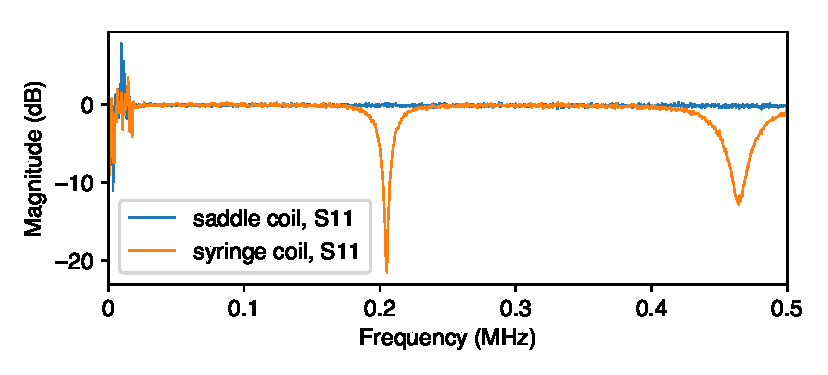
\includegraphics[width = 0.95\textwidth]{/figures/experiments/lowFieldSpectrometer/networkAnalysis.pdf}
                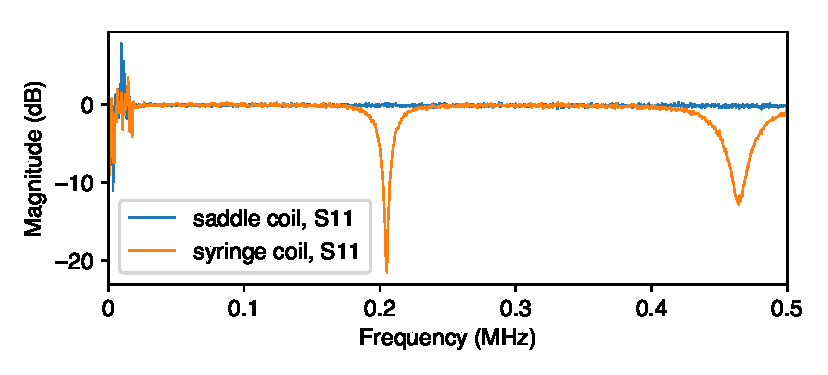
\includegraphics[width = 0.99\textwidth]{/figures/experiments/lowFieldSpectrometer/networkAnalysis.pdf}
            \caption{Network analysis Frequency of a receive coil (orange) and saddle transmit coil (blue) commonly used in the low field experiments and a correspinding transmit coil. Note the strong dip in the syringe receive coil at around \SI{210}{\kilo\hertz} that was intended to receive the NMR signal as well as the second, lower and braoder resonance at around \SI{470}{\kilo\hertz}. In contrast to that, the broadband transmit coil displayed in blue shows a flat frequency response.}
                \label{fig:results:networkAnalysis}
            \end{figure}
            \begin{figure}
                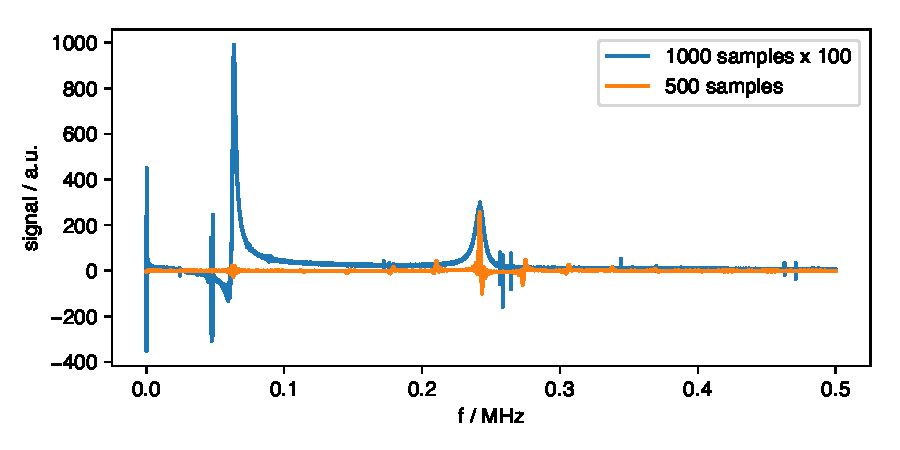
\includegraphics[width = 0.95\textwidth]{/figures/experiments/lowFieldSpectrometer/niNetworkAnalysis.pdf}
                \caption{ADC result of a pulse transmitted to the tuned receive coil. the central peak shows the resonance frequency of the coil. Similar to the actual network analysis measurement, the lower  order resonance can be seen to the right at around \SI{70}{\kilo\hertz}. Note the stron frequency shift due to the different downstream receive circuit.}
                \label{fig:results:niNetworkAnalysis}
            \end{figure}
            For the measurement with the National Instruments card, a string frequency shift of the two peaks is observed. The peak intended for singnal reception is shifted to frequencies of around \SI{70}{\kilo\hertz} while the peak to its right is shifted to \SI{240}{\kilo\hertz}. This resonance was then used for subsequent measurements. Dual resonant coils for 1H and 13C signal reception showed a less prominent dip in both channels, while the additional channel (1H in most cases) \todo{ref methods} was affected more strongly by the adapted circuitry.
        \subsubsection{$\mathbf{B_0}$ coils}
        The manufactured $\mathrm{B_0}$ coils show fields (i.e. frequencies) as well as  linewidths in the order of magnitude the simulations predicted (section \ref{sec:results:sim}). Through manufacturing errors, and changes to the coil in long term use cases, the linewidths deteriorated. It is important to note that, at currents above $\SI{1}{\ampere}$, the $\mathrm{B_0}$ coil heated noiticabely. While the heating itself is unproblematic, the resulting exansion of the materials leads to an overall longer coil and thus lower fields \ref{fieldSolenoid}.     \subsection{Shims and programmable power supply}
        The three linear shims are adjustable via the programmable power supply and show their expected effect. The rotational position of the receive coil is relevant to the shims indicating they're working as intended (i.e. x- and y-shim currents need to be exchanged while z shim remains unchanged on a \SI{90}{\degree} rotation) . Manual shimming results are shown in figure \ref{chap:MaterialsAndMethods:lowFieldSpectrometer:shims}. The optimal results were achieved for currents of \SI{0}{\milli\ampere},  \SI{0}{\milli\ampere} and \SI{0}{\milli\ampere} for x-, y- and z-shim respectively. Using the added shim tool \todo{methRef}, line widths were reduced from $\approx \SI{250}{\hertz}$ to $\approx \SI{30}{\hertz}$ in the case of large samples of $\approx $\SI{40}{\milli\litre}. If the initial field was generated by a less homogeneous, more asymmetric coil in which no signal was visible without shims, signal was discovered and linewidths went down to $\approx \SI{50}{\hertz}$.
        \begin{figure}
            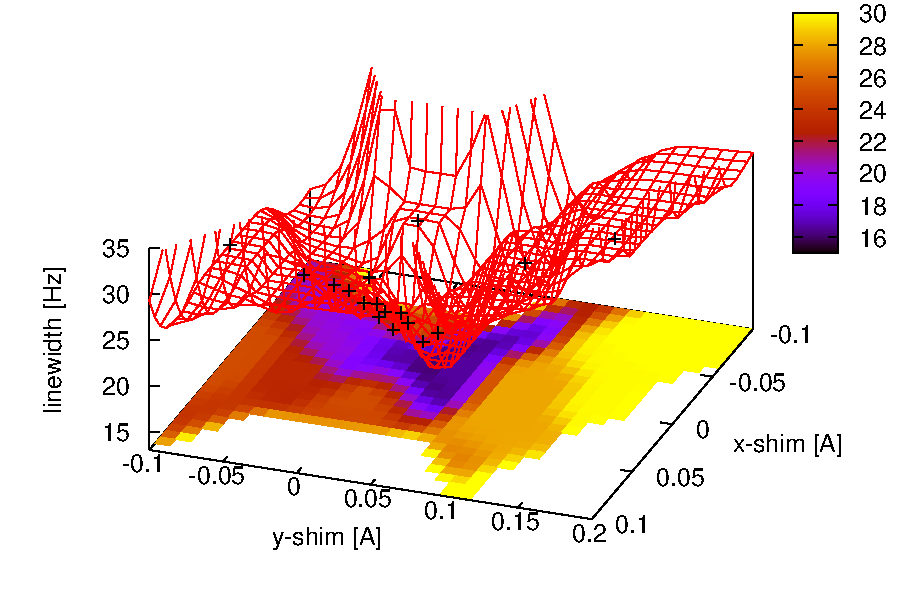
\includegraphics[width=0.99\textwidth]{/figures/experiments/lowFieldSpectrometer/shims/shimXY.pdf}
            \caption[Manual low field shimming]{Linear shimming in x- and y-directions. Shimming was done manually: 1H spectra of water were recorded and evaluated as to their linewidth. Later, automatic shimming was implemented (see section \ref{chap:MaterialsAndMethods:lowFieldSpectrometer:shims}). Black dots indicate actual measuremet points, the red mesh is a spline interpolation of the measurement data. The same interpolation is shown as a colormap on the bottom of the graph where black color corresponds to narrowest lines and thus highest homogeniety.}
            \label{fig:results:lowFieldSpectrometer:shims}
        \end{figure}
        The automatic discovery of the linewidth of a given measurement works well and yields results similar to the ones of a manual adjustment with a lot less user interaction. The fast fittingless linewidth detection based on interpolation yields linewidths within \SI{10}{\percent} of the fitted result if the SNR is sufficient, i.e. the maximum value can clearly be attributed to the water resonance.
    \subsection{Sabre shuttling system}
        The system designed to transfer a sample between fields works as intended. Fluid losses are small and thus
        acceptable with about \SI{25}{\percent} lost within \~15 shuttling cycles at high flow rates of \SI{20}{\litre
        \per\hour} and long bubbling times of 30 seconds per measurement i.e. \SI{8}{\minute} of pH2 flow through the
        sample. The bubbling system works well and provides pH2 to the solution in amounts large enough to generate
        polarization levels in the single digit percent range \ref{fig:results:highlyPolarized15Nspectrum}.
        \subsubsection{15N coil}
        The coil for 15N signal reception was matched and tuned to fit the requirements of the system. The network analyzer showed a q-factor of \todo{n} and a width of nn. Inside the small animal NMR, similar resonance widths of nn were observed while the attenuation was \SI{1}{\deci\bel}. Clear signal was visible using the 15N glycine phantom in a single shot measurement. Shimming reduced linewidths of the phantom to \SI{10}{\hertz}. Linewidths of the hyperpolarized 15N pyridine signal were in the range of \SI{30}{\hertz} without explicit shimming for its geometry and content.
            \begin{figure}
                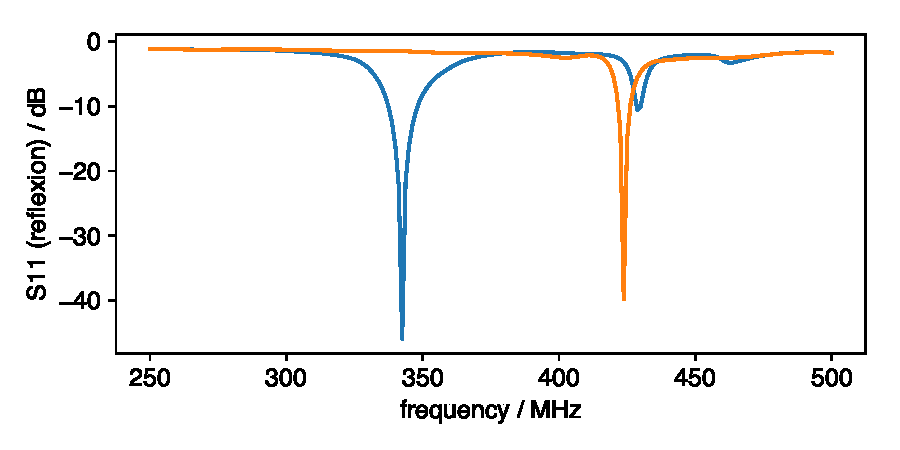
\includegraphics[width=0.99\textwidth]{/figures/experiments/15NSabre/15Ncoil.pdf}
                \caption[15N coil network analysis]{The range of frequencies covered by the 15N solenoid coil built for the hyperpolarized experiments. Due to the large range of the tune capacitor, the range was large enough to cover \SI{100}{\mega\hertz} with matching capacities in the \SI{40}{\deci\bel} range.}
                \label{fig:results:15N:networkAnalysisCoil}
            \end{figure}
        \subsubsection{Flip angle calibration}
            The flip angle for the $^{15}N$ coil was not automatically calibratable which is why it was manually calibrated. The example shown here uses a 
            \begin{figure}
                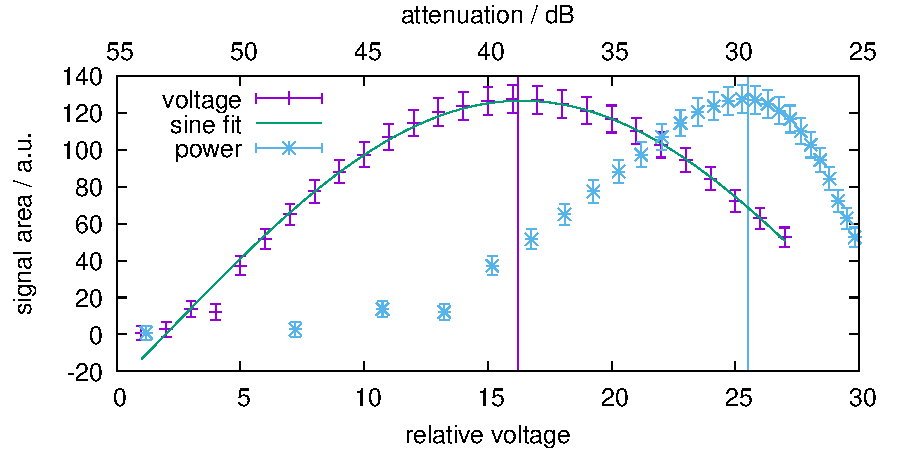
\includegraphics[width=0.99\textwidth]{/figures/experiments/15NSabre/flipAngle/faDiss.pdf}
                \caption{Signal area of the $^{15}N$-Glycine phantom measured in the $^{15}N$ coil plotted over relative voltage and attenuation. The plot over relative voltageis fit with a sine to find the \SI{90}{\degree} flip angle. The \SI{90}{\degree} angle is marked by a vertical line for both the voltage and attenuation plot.}
                \label{fig:results:15N:flipAngle}
            \end{figure}
        \subsubsection{Parahydrogen supply - bubbling}
            The newly constructed bubbling disk showed to provide hydrogen more homogenously than the previously used single hole supply. Different hole sizes provide similar flow for samples of different viscosities. The widening cylinder provides enough spcae for bubbles to burst and reduce losses due to fluid splashing into the venting line.
        \subsubsection{Pressure stability}
            The pressure stability of the vessels has been simulated to withstand \SI{200}{\bar} . I decided using a factor of safety of $\gamma = 4$. As expected, the most vulnerable part is the long side of the cylinder, but wall thickness of \SI{3}{\milli\meter} suffices for a factor of safety of 4 if the setup is operated at a maximum pressure of \SI{50}{\bar}.Experimentally, the pressure resistance of \SI{50}{\bar} was confirmed; no problems concerning material fatigue were observed whatsoever within a few thousand pressure cycles. Figure \ref{fig:results:bubblingReactorPressure} shows the displacement of the different parts at \SI{200}{\bar}. The maximum displacement is in the range of \SI{0.25}{\milli\meter} and is within the yield strengths of PSU.
            \begin{figure}
                \centering
                \subfloat[Overall displacement\label{fig:results:sim:pressure:yDisplacement}]{\includegraphics[width = 0.49\textwidth]{/figures/simulations/15NSabre/displacement200.eps}}
                \hfill
                \subfloat[X displacement\label{fig:results:sim:pressure:xDisplacement}]{\includegraphics[width = 0.49\textwidth]{/figures/simulations/15NSabre/xDisplacement200.eps}}\\
                \subfloat[Y displacement\label{fig:results:sim:pressure:yDisplacement}]{\includegraphics[width = 0.49\textwidth]{/figures/simulations/15NSabre/yDisplacement200.eps}}
                \hfill
                \subfloat[Z displacement\label{fig:results:sim:pressure:zDisplacement}]{\includegraphics[width = 0.49\textwidth]{/figures/simulations/15NSabre/zDisplacement200.eps}}
                \caption[Reactor wall stress simulations]{Wall stress of the low field reactor for pressure levels at \SI{200}{\bar}. (a) shows the overall displacement while (b), (c) and (d) show the displacement in X-, Y-, and Z-direction.  The yellow arrows shown in pairs of four indicate the areas pressure was applied to in the simulation.}
                \label{fig:results:bubblingReactorPressure}
            \end{figure}
            Chemical resistance to methanol- and ethanol-pyridine mixtures was as good as expected, though resistance to pure pyridine is not given. While there was never any problem with the pyridine concentrations  up to \SI{30}{\micro\Molar} used in the experiments, a neat pyridine batch showed to dissolve the PSU casing.\todo{ref discussion, other materials}
        \subsubsection{Mu metal shielding}
            The three layered mu metal shield reached fields of \SI{50}{\nano\tesla} insisde the stray field of the \SI{9.4}{\tesla} small animal MRI. In earth magnetic field, fields inside the shield went down even further to \todo{measure}.Manual degaussing was prone to errors and left the shields in different, non-comparable states. The workshop-built automatic degaussing power supply was capable of reducing those errors and generate a field of \SI{50}{\nano\tesla} reproducibly.The slew rate of \SI{0.25}{\ampere\per\second} showed to be sufficient in combination with an initial current of \SI{7}{\ampere}. The adaption to other shield sizes works automatically after a single calibration run.
        \subsubsection{Low field manipulation}
        The field inside the Mu Metal shielding was measured without any current flowing in the B0 coil as well as with the coil turned on. Measurements showed different results for the solenoid coil used in the beginning and the later used helmholtz coil. Both coils were used to measure fields at the reactors position. As field steps using the power supply directly were in the range of \SI{213\pm 31}{\nano\tesla} per \SI{0.1}{\milli\ampere}, the lowest settable current, an additional \SI{10}{\kilo\ohm} resistor was used to reduce the current by a factor of 1000. The source was not usable in constant current mode, thus the voltage was set introducing a larger error to the current, but allowing for very precise adjustments to the current. Results that show the highly linear dependence of current (or voltage, ohmsch dep.) and magnetic field are shown in figures \ref{} and \ref{figures:results:helmholtzCoilsCenterField}. The slope of the voltage-field line is steeper for the solenoid coil as shown in the inset of figure \ref{}. $B_{xy}$ is small compared to $B_z$ over the complete range displayed. This leads to a dependence between voltage and field of
        \begin{equation}
            B(U) = 111.3\pm 0.1 \si{\nano\tesla\per\volt} - 79.1 \si{\nano\tesla}
        \end{equation}
        for the Helmholtz coil and
        \begin{equation}
            B(U) = 333.3 \frac{\si{\nano\tesla}}{\si{\volt}} - 168 \si{\nano\tesla}
        \end{equation}
        for the solenoid coil. The slope for the solenoid coil is larger 
            \begin{figure}
                \centering
                \label{figures:results:helmholtzCoilsCenterField}
                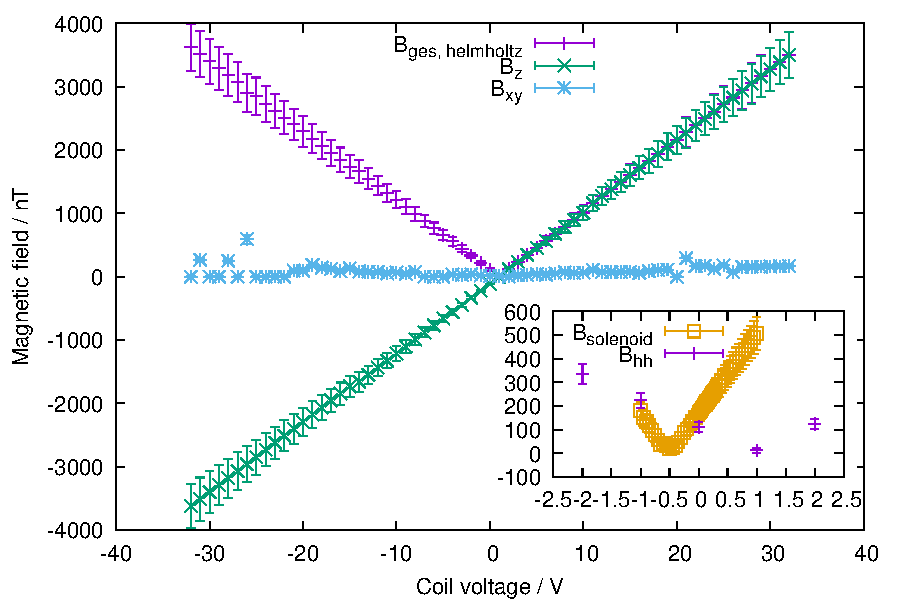
\includegraphics[width=0.99\textwidth]{/figures/experiments/helmholtzCoils/fieldHelmholtzCoils.pdf}
                \caption{Calibration of the voltage (and thus current) to reference actual fields using the fluxgate sensor and ramping trough the voltages in both polarities. In the insert, the fields of the previously used solenoid coil can be seen in comparison to the helmholtz coils' field in the central region. Its slope is steeper than the helmholtz coils'. oltage applied to the inner Helmholtz coil pair via a \SI{10}{\kilo\ohm} resistor to limit currents to values below the power supply's resolution.}
            \end{figure}
            
        \subsubsection{Shuttling reproducibility}
        \label{results:15N:shuttlingReproducibility}
            To ensure that the sample is removed completely from the high field side, spectra in both 'states' of the system were recorded (Figure \ref{fig:results:15N:shuttlingRemoval}). The residue left in the high field chamber after the shuttling procedure does not generate significant signal, but after maximizing the noise integral through phase shifts, the ratios upper limit $\frac{I_{in}}{I_{out}}$ can be estimated and corresponds to a maximum fluid volume of \SI{0.05}{ml}remaining in the high field chamber. Considering this fraction completely non-polarized, the overall polarization of a \SI{3}{ml} sample will be reduced by \SI{9999}{\percent} \ref{fig:results:15N:shuttlingReproducibility}.
            \begin{figure}
                \centering
                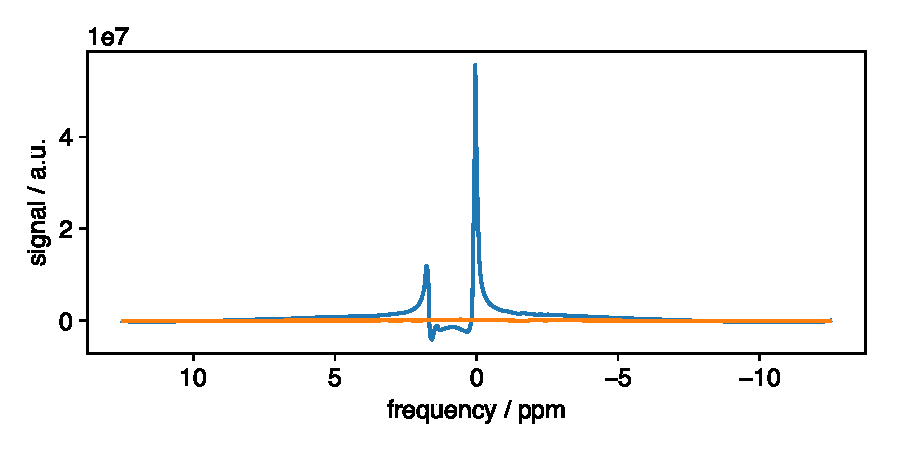
\includegraphics[width=0.99\textwidth]{/figures/experiments/15NSabre/reproducibility/spectraComparisonShuttle.pdf}
                \caption[High field removal efficiency]{1H spectra of the high field reactor in the filled (blue) and empty (orange) state. The filled state delivers a lot more signal as expected while the integration over the empty state spectrum shows a signal reduction of 1000.}
                \label{fig:results:15N:shuttlingRemoval}
            \end{figure}
            To test the reproducibility of the shuttling system, a hyperpolarized 1H pyridine sample was shuttled back and forth multiple times. The results of the measurement are shown in figure \ref{fig:results:15N:shuttlingReproducibility}. It can be seen that even in the setting used for testing with high flows of \SI{40}{\litre\per\minute} and extensive bubbling of \SI{30}{\second} per measurement cycle, the signal drops to only \SI{75}{\percent} after 15 shuttling procedures. Note that the actual losses may be even smaller as temperature effects are neglected in this measurement, but have been shown to have an effect on signal intensity in seperate experiments.
            \begin{figure}
                \label{fig:results:15N:shuttlingReproducibility}
                \centering
                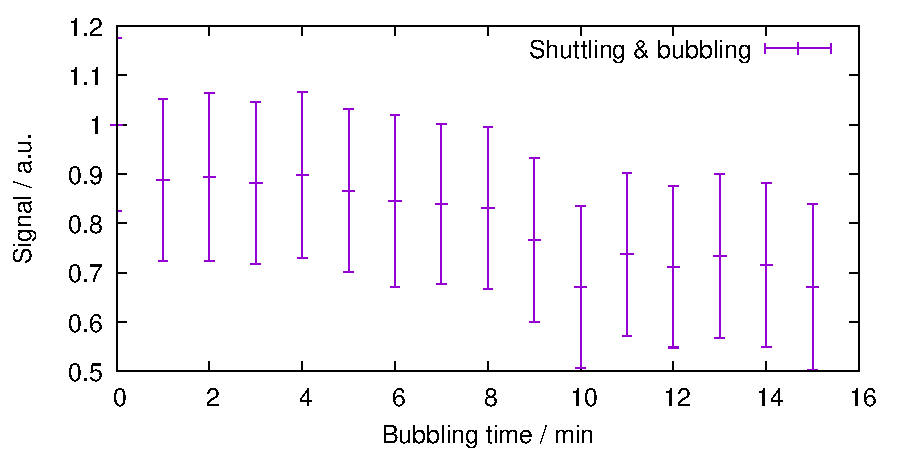
\includegraphics[width=0.99\textwidth]{/figures/experiments/15NSabre/reproducibility/bubblingLosses.pdf}
                \caption[Bubbling fluid losses]{Signal intensity during multiple minutes of hydrogen bubbling using a hyperpolarized 1H-pyridine sample. Note that the signal drops to about \SI{70}{\percent} of its initial value after 8 minutes of continuous hydrogen supply. The initial rise of signal during the first two minutes indicates a temperature effect unaccounted for.}
            \end{figure}
    \subsection{Fluxgate readout electronics}
        The readout electronics were designed to feature a wide range of amplifications for all three spatial dimensions. A 24 V DC power supply was fitted with a DC-DC-converter to provide the $\pm\SI{15}{\volt}$ to power the Fluxgate. Additionally the PCB board was fitted with the electronic parts (see \ref{sec:methodsFluxgate}). For testing purposes, a simple program using serial in and output to toggle the analog switches was written. All switches were successfully tested to work, though three had to be replaced at some point for malfunction.  Apparently this was due to damage during assembly as the board is now working as expected.
    \subsection{Fluxgate calibration}
        The three spatial channels of the fluxgate sensor needed to be calibrated as to their intrinsic offsets as described in \ref{materialsMethods}. Data for X- and Y-channels are shown in figure \ref{fig:results:fluxgate:xysinus}.
        \begin{figure}
            \label{fig:results:fluxgate:ysinus}
            \centering
            
\includegraphics[width=0.99\textwidth]{/figures/experiments/fluxgate/xField.pdf}
            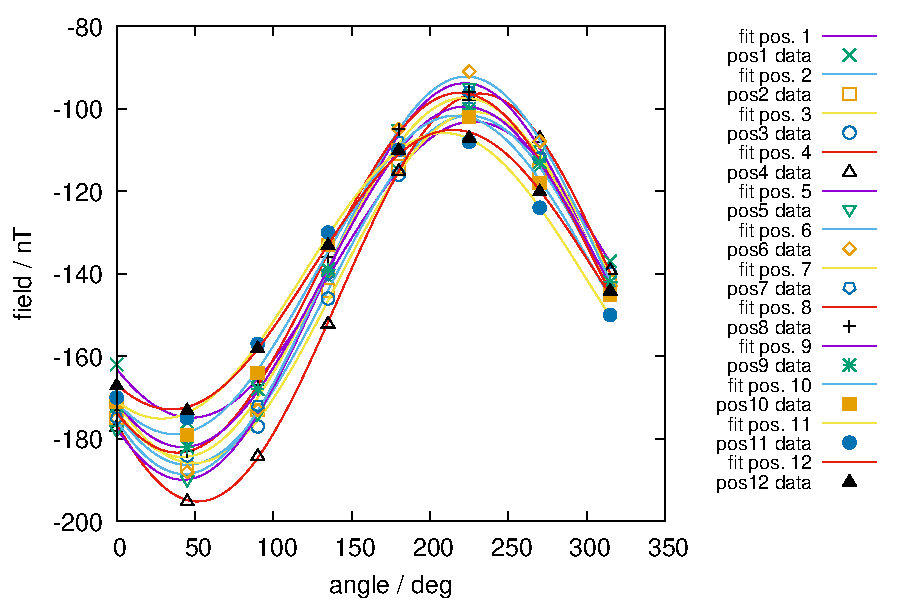
\includegraphics[width=0.99\textwidth]{/figures/experiments/fluxgate/yField.pdf}
            \caption[Calibration results X/Y]{Calibration data of X- and Y-channel. Each dataset in the key
            corresponds to a full rotation at one position in the MuMetal shield. The solid lines correspond to
            a sine fit to each dataset with phase, amplitude and offset as fitting parameters. Error bars are not
            displayed for better visibility.}
        \end{figure}
        The fit parameters shown in table \ref{table:results:calibrationFitParams} allow for calibration of X- and Y- channel by calculating the average offset for all Positions.
        \begin{table}
            \centering
            \label{table:results:calibrationFitParams}
            \begin{tabular}{r|cccccccccccc}
                \label{table:results:calibrationFitParams}
                position & 1& 2 & 3 & 4 & 5 & 6\\
                \hline
                amplitude & 22.4 & 27.0 & 35.9 & 39.6 & 45.2 & 42.5\\
                offset \\
                phase \\
                \hline
                position & 7 & 8 & 9 & 10 & 11 \\
                \hline
                amplitude & 42.9 & 45.1 & 45.4 & 44.6 & 40.6\\
                offset \\
                phase
            \end{tabular}
            \caption[Fluxgate calibration results]{Calibration results at different positions of the fluxgate inside the mu metal shield. See figure \ref{fig:results:fluxgate:plotSpatial} for a comprehensive visualization of those results. Figure \ref{fig:materialsMethods:muMetalsizes}\todo{add ref} shows the dimensions and positions of the setup.}
        \end{table}
        \begin{figure}
            \label{fig:results:fluxgate:zcal}
            \centering
            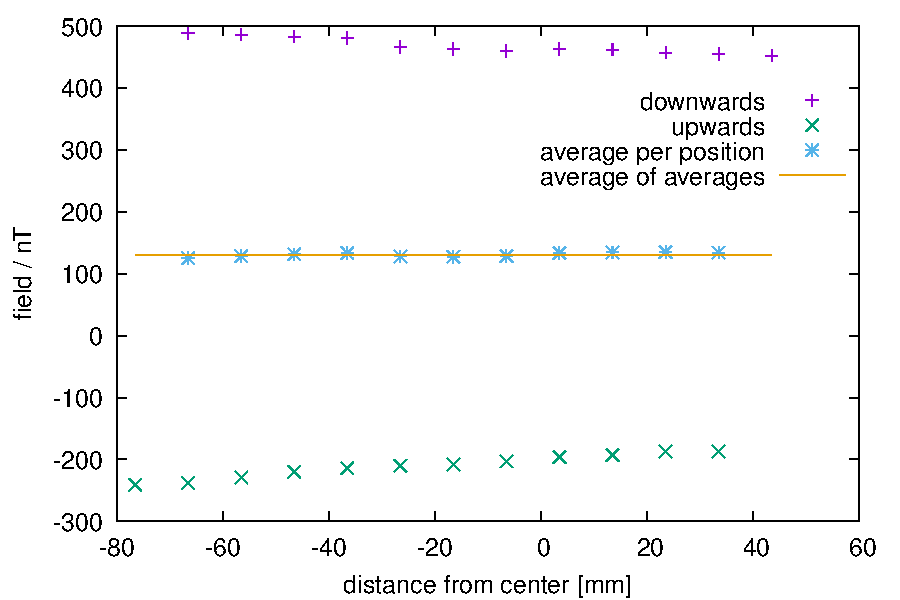
\includegraphics[width=0.99\textwidth]{/figures/experiments/fluxgate/zField.pdf}
            \caption[calibration results Z]{Calibration of the Z-channel. Due to spatial limitations, no full rotation in z direction was possible. The two datasets represent one measurement in "upwards" ond one in "downwards" direction. The solid line represents the average of the positional averages of the two directions.}
        \end{figure}
        Using the data for calibration, the measurements of the X- and Y-channels can be used to plot a 2D-section of the field using the phase of the fit as the field direction and the amplitude as its magnitude. Both X- and Y-sensor are shown in figure \ref{fig:results:fluxgate:plotSpatial2d}. The absolute positions are indicated in the figure to enable comparison of the individual results in the same absolute position. The same data is also shown in a 3D plot (fig. \ref{fig:results:fluxgate:plotSpatial3d}) to show the field progression inside the mu metal shield.
        \begin{figure}
            \label{fig:results:fluxgate:plotSpatial3d}
            \centering
            %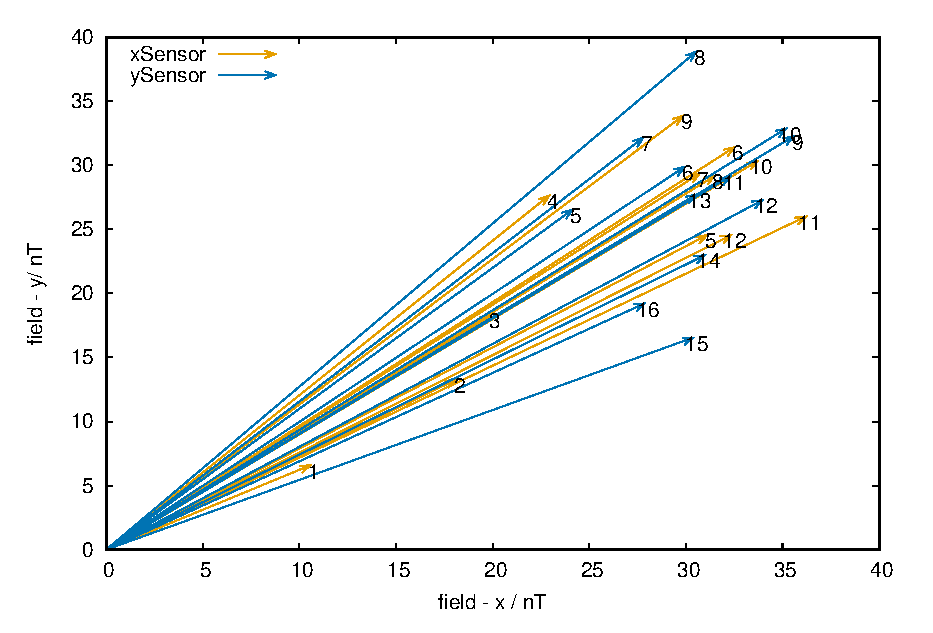
\includegraphics{/home/philipp/Documents/thesis/figures/experiments/fluxgate/spatial2dProjection.eps}
            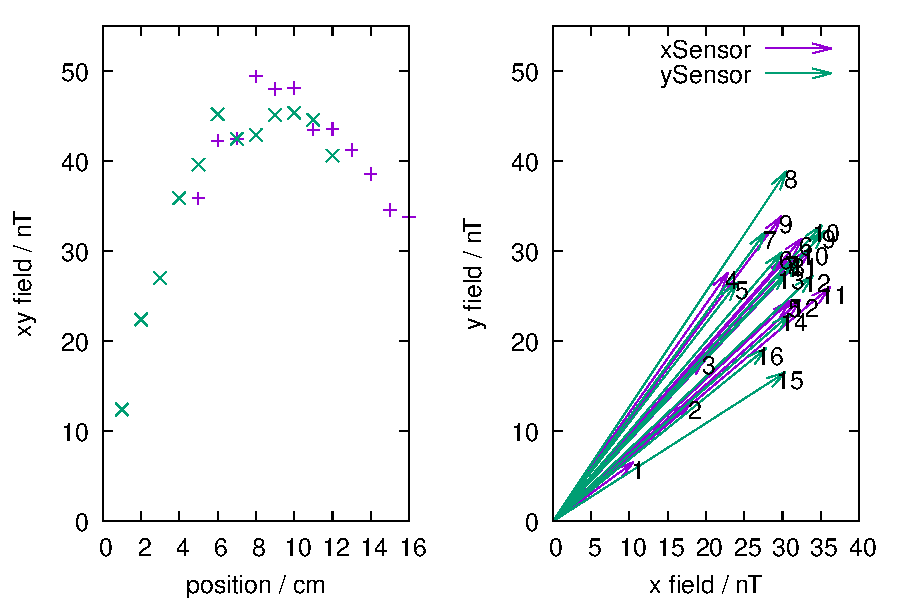
\includegraphics{/figures/experiments/fluxgate/spatial2dProjection.pdf}
            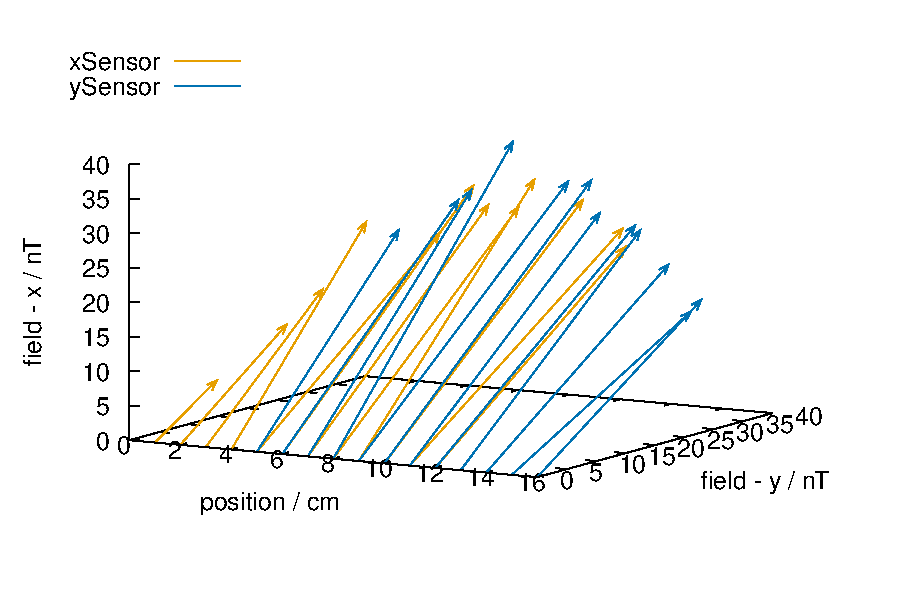
\includegraphics{/figures/experiments/fluxgate/spatial3d.pdf}
            \caption{Results of the fluxgate calibration visualized: on top, the two projected views are shown that visualize the absolute field values in the x-y-plane and the field's direction. The field reaches a maximum in the center of the shield at around \SI{8}{\centi\meter}. The angle of the field remains fairly constant within an angle of $\approx$ \SI{30}{\degree}. In the lower part, the same data is shown as a 3d plot for a better overview.}
        \end{figure}
\section{Measurements}
    \subsection{Low field NMR}
    \label{chap:results:lowFieldNMR}
        Low field spectra were acquired using different setups. The main modification between setups concerned the $B_0$ coil. The initially used solenoid coil showed linewidths of about 0.5 - \SI{1}{\kilo\hertz}. Due to mechanical destruction of one coil and those rather wide lines, a new coil design was simulated and built \ref{fig:results:compensationWindOptimization} using Biot Savart calculations. While currents to generate the same field were higher by a factor of about 2, field homogeniety improved greatly and now shows linewidths of about \SI{21}{\hertz} (figure \ref{results:lowFieldSpectrometer:thinLine}). Flip angle calibrations for different pulse durations were calibrated and yielded the results shown in table \ref{table:results:FA}. These results were used in successive measurements with the low field NMR unless stated differently.
        \begin{table}
            \centering
            \begin{tabular}{ccccc}
                pulse duration [ms] & 200 &  400 & 800 & 1200 \\
                $\mathrm{V}_{\SI{90}{\degree}}$ [V] & & & & 
            \end{tabular} 
            \label{table:results:FA}
            \caption{Results of the manual flip angle calibration using the saddle excitation coil and the syringe receive coil for pulse durations ranging from 200 to 1200 ms and block pulse shape.}
        \end{table}
            \begin{figure}
                \centering
                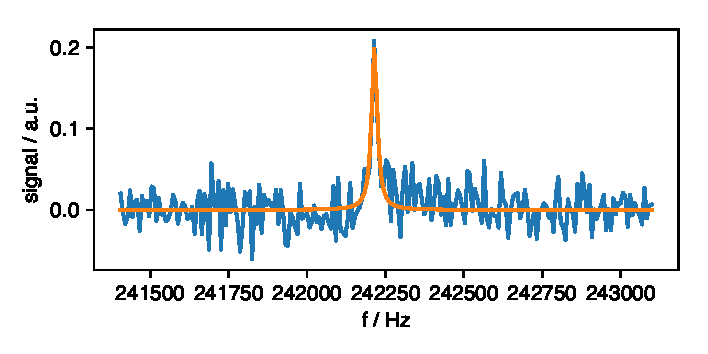
\includegraphics[width = 0.99\textwidth]{/figures/experiments/lowFieldSpectrometer/helmholtzNarrowLine.pdf}
                \caption{A $_1\mathrm{H}$ line of a Magnevist doped water sample inside the 'syringe coil'. Linewidth is down to \SI{21}{\hertz} in this example without the use of shim coils.}
                \label{results:lowFieldSpectrometer:thinLine}
            \end{figure}
    \subsection{Sabre in water}
    For measurements of continuously hyperpolarized nicotinamide in deuterated water, the buildup of hyperpolarization was observed by TR variation. The results of these measurements are shown in figure \ref{results:lowFieldSpectrometer:SabreInWater:TRVariation}. TR was varied from \SI{1}{\second} to \SI{30}{\second}, the signal was stronger for longer TR and thus longer buildup time. The difference between TR~=~\SI{15}{\second} and TR~=~\SI{30}{\second} is already within the margin of error and implies that a plateau is reached in this domain. Note that a dummy scan was necessary for each TR measurement series to deplete the previously built hyperpolarization. The effective buildup rate can be calculated from these results (table \ref{table:results:TRvariation)}) and is shown in figure \ref{results:lowFieldSpectrometer:hpBuildup}. Using this data, the specific buildup rate, i.e. an effective $T_1$ was determined to be \SI{5.4\pm 0.2}{\second}. Similarly, for $H_2O$, a lower $T_1$ of \SI{2.4\pm0.2}{\second} was found at the \SI{5}{\milli\tesla} field.
        \begin{table}
            \centering
            \begin{tabular}{|c|ccccccccc|}
                \hline
                TR [s] & 1 & 2 & 3 & 4 & 6 & 8 & 10 & 15 & 30 \\
                \hline
                signal [a.u] & 1 & 2\\
                standard deviation [a.u.] & 0.1 & 2\\
                \hline
            \end{tabular}
            \label{table:results:TRvariation}
            \caption{Average signal of each TR measurement series excluding the dummy scan destroying previously accumulated polarization. Standard deviation is additionally given.}
        \end{table}
        \begin{figure}
            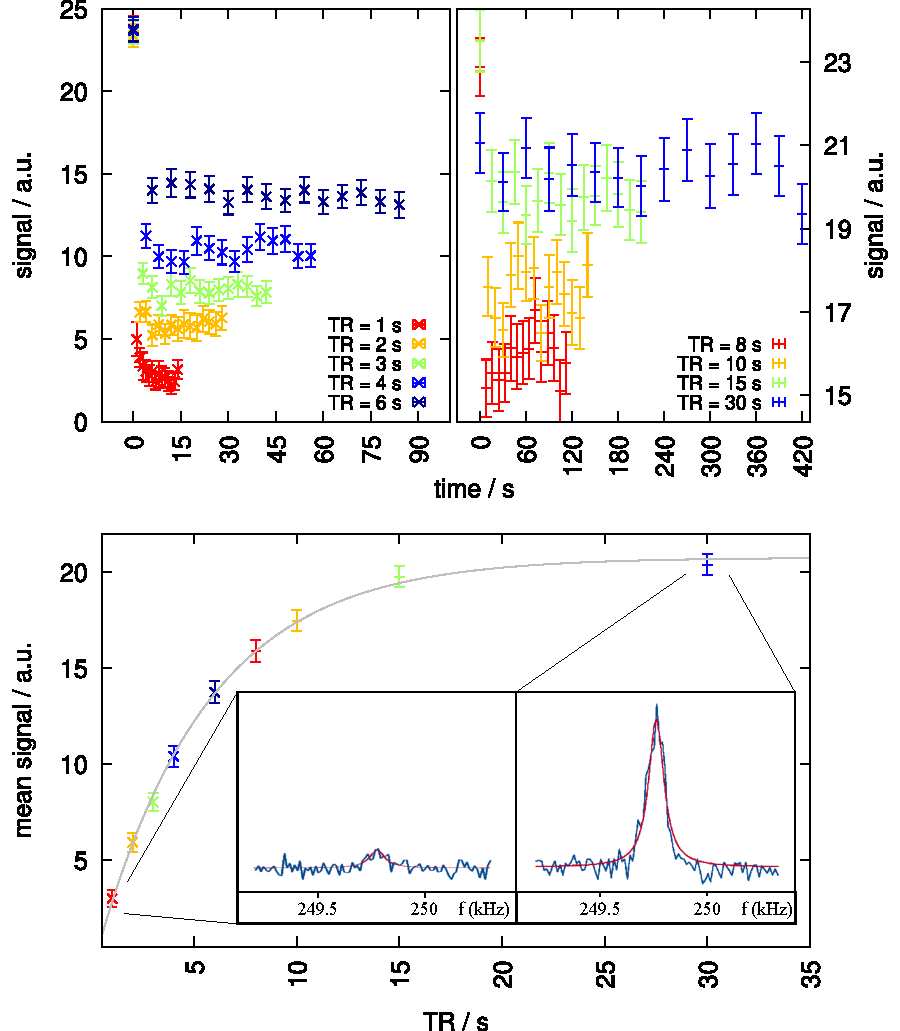
\includegraphics[width=0.99\textwidth]{/figures/experiments/lowFieldSpectrometer/inSituSabreWater/combinedInsert.pdf}
        \caption{Variation of the TR in continuously hyperpolarized sample of IR-IMes, nicotinamide and D$_2$O. Each TR was measured 10 times, resulting in varying cumulative measurement times. Note that one 'dummy scan' was necessary to reach the steady state for each TR, to be seen at timepoint 0. Average values increase with TR and correspongdingly longer buildup rates. Bottom: The average values except for the first, which is out of steady state equilibrium, for each TR over TR. An exponential function was fit to the data revealing a buildup rate, i.e. an effective $T_1$ of \SI{5.4\pm 0.2}{\second}}
        \end{figure}
    \subsection{Imaging of contiuously hyperpolarized solution}
    Using the Magritek Terranova, images of continuously hyperpolarized solutions were acquired. Using the watery Sabre solutions, imaging at low fields, specifically even at earth magnetic field, were possible, if previous to imaging prepolarization or, in this case, hyperpolarization fields of $\approx$ \SI{5}{\milli\tesla} were used. The results of such an image at earth magnetic field is shown in figure \ref{fig:results:earthFieldImage}. For the image, a polarization of \todo{calc} was calculated. The SNR of the much lower conscentrated nicotinamide \SI{1.3}{\milli\Molar} corresponding to \SI{12}{\milli\gram} nicotinamide in \SI{5}{\milli\litre} D2O) was higher than that of a much higher consentrated and larger volume doped water sample (\SI{20}{\milli\litre} of \SI{55}{\Molar} water) which showed SNR of 4.7.  \begin{figure}
            \label{fig:results:earthFieldImage}
            \includegraphics[width=0.9\textwidth]{/figures/experiments/earthFieldImaging/2dImagePlusOutline}
            \caption[Earth field Sabre image]{An image of a continuously hyperpolarized sample and a Gadolinium doped water reference acquired at earth magnetic field after prepolarization for \SI{30}{\second}. The much lower concentrated nicotinamide sample (\SI{1.3}{\milli\Molar}) shows higher signal than the thermally polarized water (\SI{55}{\Molar}), though water is also prepolarized at \SI{5}{\milli\tesla}. Resolution is (\SI{1.6}{\milli\meter})$^2$ with an acquisition time of \SI{5}{\minute} \SI{20}{\second}.}
        \end{figure}
        Linewidths in single shot experiments after shimming were in the \SI{1}{\hertz} range and thus more narrow than the low field spectrometer's lines of equal molecules.
    \subsection{Sabre in cell solution and blood}
        Measurements in pure water yielded sufficient signal to try more biologically relevant substances. Cell culture solution (PTSD) was the first step forward and showed to already significantly reduce the polarization yield. Addition of \SI{0.5}{\milli\litre} of PTSD reduced the signal by a factor of 3. This already indicated that with human blood as an addition to the solution, the performance would not be better if not worse. Measurements confimed this suspicion, the signal showed to drop by a factor of \~8 after injection of 0.3 ml of human blood into the solution already. Adding \SI{0.5}{\milli\litre} of blood completely diminishes the signal. SNR for these measurements was comparably low to begin with where
        \begin{figure}
            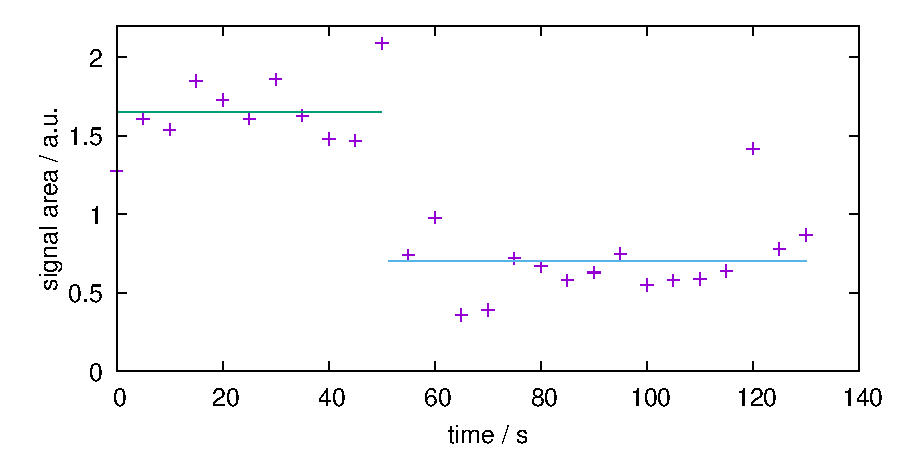
\includegraphics[width=0.99\textwidth]{/figures/experiments/lowFieldSpectrometer/inSituSabreWater/timeSeriesCellCultureSolution.pdf}
            \caption[Cell culture solution addition to hyperpolarized signal]{Time course of the signal intensity (peak height) when adding cell culture solution to a continuously hyperpolarized solution of IrIMes, pyridine and MeOD. Note the strong signal drop after addition of \SI{0.5}{\milli\litre} of cell culture solution to the sample. The straight and dashed lines indicate the average before and after addition.}
            \label{chap:MaterialsAndMethods:bloodInjection}
        \end{figure}
        \begin{figure}
            \centering
            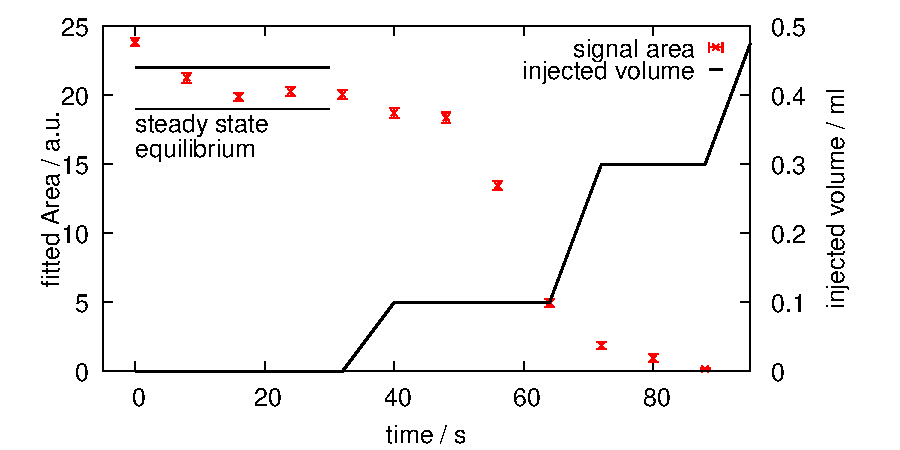
\includegraphics[width=0.99\textwidth]{/figures/experiments/lowFieldSpectrometer/inSituSabreWater/signalVariation.pdf}
            \label{chap:MaterialsAndMethods:bloodInjection2}
            \caption[Blood addition to hyperpolarized signal]{Signal drop during the injection of \SI{0.5}{\milli\liter} of blood into the solution providing hyperpolarized signal which was permanently provided with fresh pH2. First measurements show a slight drop until a steady state is reachd. The steady state then loses signal intensity as the amount of substance injected is increased.}
        \end{figure}
    \subsection{Liposomes and Sabre}
        The results of cell culture solution and human blood addition to a working, hyperpolarized sample suggested that other approaches were necessary to achieve hyperpolariation in biologically relevant surroundings. The previously described method of encapsulation of substrate and catalyst in double layered liposomes. While the liposomes formed, the size distribution according to the lipochemists was broader than usual. \todo{plot results if available} The experiments trying to hyperpolarize the liposomal structures failed and it showed that the addition of the components used in the generation of liposomes into a working hyperpolarized solution already depleted the signal to a non-detectabel level. Different solvents and substrates were tested in combinations but did not yield any observable signal.
    \subsection{15N Sabre}
        $^{15}\mathrm{N}$ labeled substances were used to generate high polarization on the substrate in \si{\nano\tesla} fields. Results are shown here and include spectroscopic as well as imaging experiments.
    \subsubsection{$\mathrm{T_1}$ and $\mathrm{T_2}$ measurements}
        Results for $T_1$ measurements are shown in figure . Fit parameters are given in table .
        The relaxation times are relevant to subsequent measurements of spectra and images and were measured for both 15N-Glycine phantom and a neat, thermally polarized 15N-Pyridine sample. $\mathrm{T}_1$ was found to be \SI{52.6\pm 2.7}{\second} for MeOH as a solvent and \SI{76.9\pm 5.6}{\second} for MeOD. $\mathrm{T}_2$ was measured to be \SI{435\pm 38}{\milli\second}.
        \begin{table}
            \begin{tabular}{|c|c|c|c|c|}
                \hline
                    & time constant / s & error / s & scaling factor & error\\
                    \hline
                $\mathrm{T_1}$ MeOH & 52.6 & 2.7 & & \\
                $\mathrm{T_1}$ MeOD & 76.9 & 5.9 & & \\
                $\mathrm{T_2}$ MeOD &  0.435 & 0.038 & &\\
                glycine phantom $\mathrm{T_1}$& & &  & \\
                glycine phantom $\mathrm{T_2}$& & & &  \\
                \hline
            \end{tabular}
            \caption[Relaxation times]{Relaxation times T1 and T2 of hyperpolarized pyridine. MeOD as a solvent increases T1 slightly and was used for subsequent measurements.}
        \end{table}
        \begin{figure}
            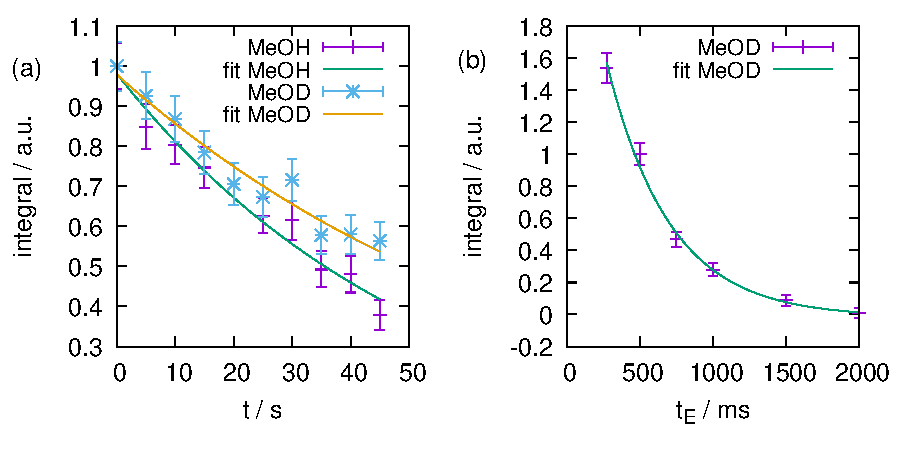
\includegraphics[width = 0.99\textwidth]{/figures/experiments/15NSabre/relaxation/T1_T2.pdf}
            \caption{$T_1$and $T_2$ relaxation times for a hyperpolarized pyridine sample. $T_1$ was measured in MeOH and MeOD. Both solvents show similar relaxation times while the deuterated solvent's is slightly longer. $T_2$ is a lot shorter than $T_1$.}
        \end{figure}
    \subsubsection{Pressure dependence}
        To see the influence of the pH2 pressure during bubbling, the same experiment was repeated multiple times at different pressures. The results of these measurements are shown in figure \ref{}. A mostly linear pressure dependence can be estimated from the data indicating that the catalytic reaction is still in the low concentration regime.
        \begin{figure}
            \label{fig:results:15N:pressureDependence}
            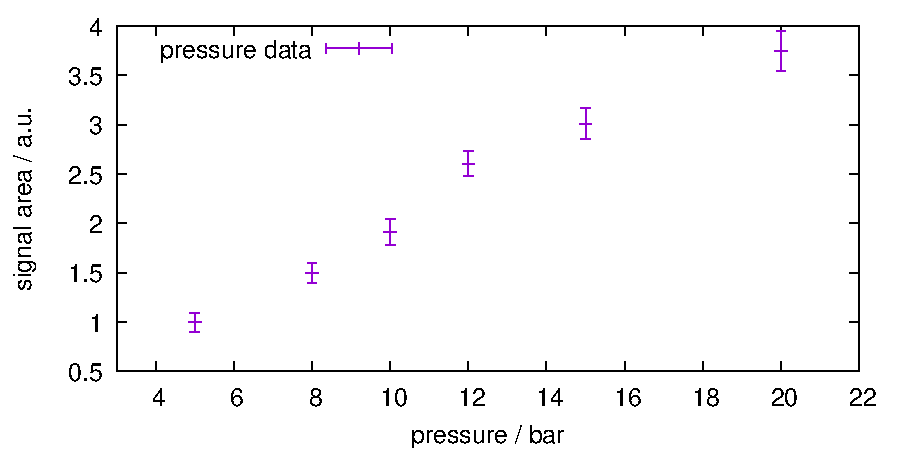
\includegraphics[width = 0.99\textwidth]{/figures/experiments/15NSabre/pressureDependence/pressureDependence.pdf}
            \caption[Pressure dependence]{Signal area of integrals at different parahydrogen pressures used for polarization. Higher pressures lead to higher signal over the pressure range shown here. A linear behavior can be estimated from the data in the range provided.}
        \end{figure}
    \subsubsection{Concentration dependence}
        The concentration and concentration ratio have an influence on the overall signal, i.e. magnetization of the sample. Here, the concentration of pyridine is lowered over the course of the measurements while the concentration of the catalyst is kept constant. The signal of the solution increases over the course of the measurements, i.e. with falling concentration but at constant amount of substance for $^{15}$N-pyridine, i.e. the polarization increased.
        \begin{figure}
            \label{fig:results:15N:concentrationDependence}
            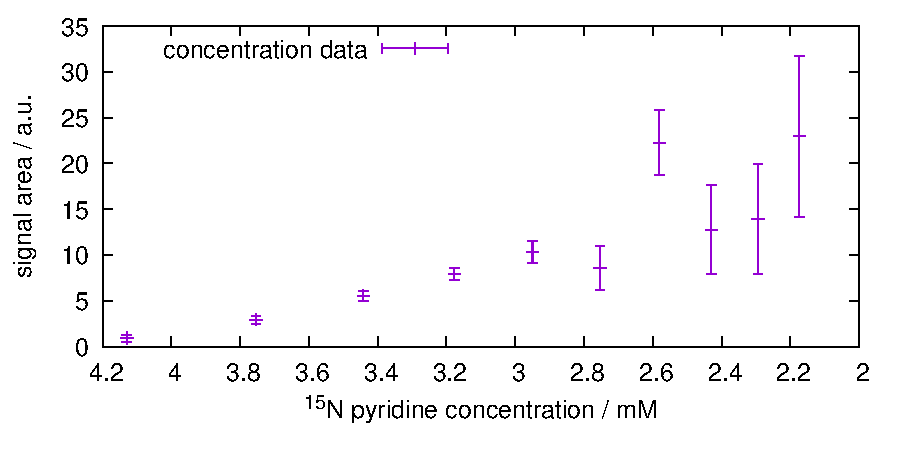
\includegraphics[width=0.99\textwidth]{/figures/experiments/15NSabre/concentrationDependence/concentrationDependence.pdf}
            \caption[Concentration dependence]{The signal of a solution of IrIMes that is diluted from left to right. Signal rises with rising dilution, i.e. with lower concentration. Concentration of catalyst is kept constant throughout the measurement.}
        \end{figure}
    \subsubsection{Flow dependence}
    Similar to pressures, flow rates have been varied to estimate their effect on the reaction's efficiency. Here, other than for the pressure measurements, flow was not a parameter linearly connected to signal intensity. As flow showed to change bubble sizes as well as the number of flow channels building, a more complex behaviour is expected and shown in figure \ref{fig:results:15N:flowDependence}. Two pressures are shown for different flow rates set at the needle valve. For both pressures, the higher flows cause higher signal up to a certain point. At \SI{10}{\bar} signal remains at constant levels from \SI{5}{\litre\per\hour}, for \SI{20}{\bar}, from a flow setting of \SI{4}{\litre\per\hour} the same effect is observable.
        \begin{figure}
            \label{fig:results:15N:flowDependence}
            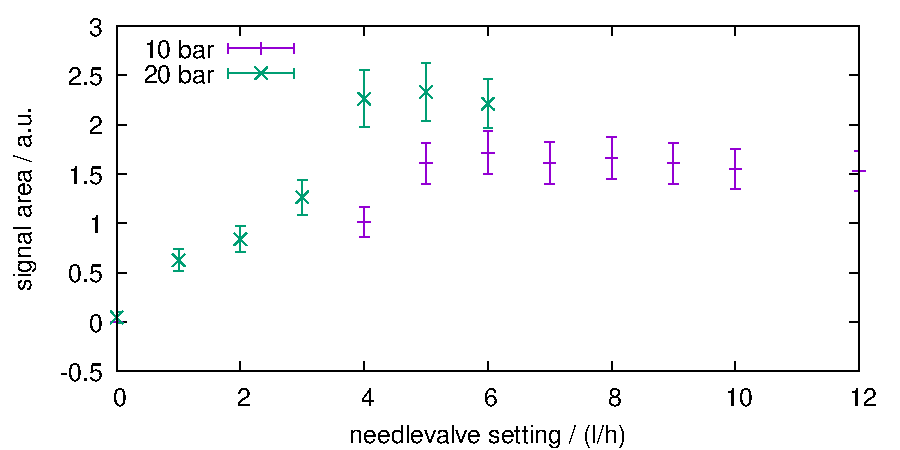
\includegraphics[width=0.99\textwidth]{/figures/experiments/15NSabre/flowDependence/flowDependence.pdf}
            \caption[Flow dependence]{The signal depending on the flow of parahydrogen through the sample at nanotesla fields. \SI{10}{\bar} and \SI{20}{\bar} pressure were measured at different needle valve settings. Higher flows first lead to higher signal, but note the flattening of the signal at high flows for both pressures.}
        \end{figure}
    \subsection{Magnetic field dependence}
        Magnetic field dependence of the polarization was measured by adjusting the field using the solenoid coil and dual helmholtz pair mounted inside the shields. The currents necessary for optimum fields were a function of the residual magnetization of the shield. Measurements of polarization and current-field correlation were conducted separately. The result shows that the field reduction generated by the shielding is large enough to surpass the optimal polarization fields as the signal drops between the two maxima that show up for two current flow directions.
        \begin{figure}
            \label{fig:results:15N:fieldDependence}
            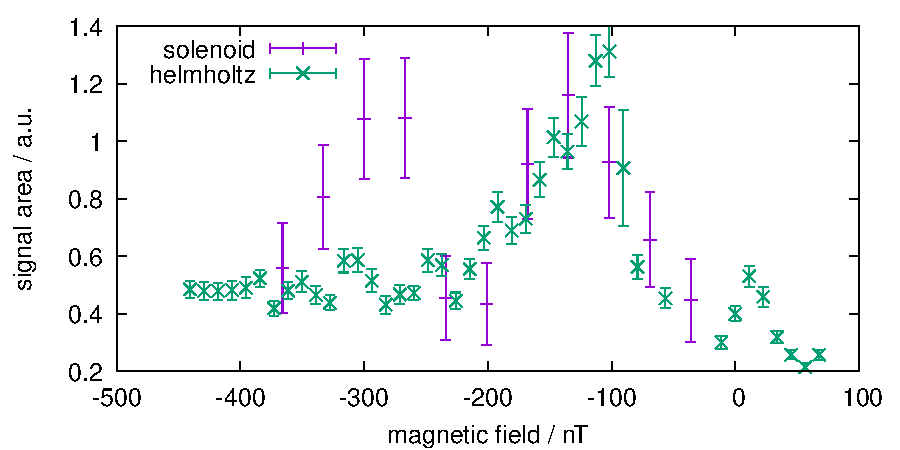
\includegraphics[width=0.99\textwidth]{/figures/experiments/15NSabre/fieldDependence/fieldDependenceCombined.pdf}
            \caption[Magnetic field dependence]{Signal over polarization field for solenoid coil and helmholtz assembly. Both coils show two distinct peaks at slightly different field strengths, the symmetry axis for the helmholtzCoil is at around \SI{30}{\nano\tesla} whereas it is around \SI{210}{\nano\tesla} for the helmholtz assembly.}
        \end{figure}
    \subsection{Polarization measurements}
        The scheme used in the first, preliminary tests provided polarizations in the range of \todo{range}. This value was drastically improved by using a more sophisticated approach, i.e. an automated high pressure shuttling system to generate high polarizations reproducibly and even at high concentrations to generate high magnetization.
    Polarizations in high concentration regimes and under otherwise optimal parameters (i.e. high flow of \SI{6}{\litre\per\minute}, high pressures of \SI{50}{\bar}, field at \SI{340}{\nano\tesla}) the maximum polarization measured was $\mathrm{P} = 4\% \pm 0.2 \%$. The parameter that was not controllable in this setup but does have a substantial influence on the magnetizatioin yield was the temperature of the sample that decreased while parahydrogen flowed through the volatile methanol used as solvent, see \ref{cd:sabreShuttling:tempControl} for a closer discussion.
        The two methods used for quantification - compariso to thermal signal, the more reliable, but very slow method, and comparison to the 15N glycine phantom, less reliable per se but fast - yield similar results if match and tune of the coil are readjusted after exchanging the sample for the phantom. This ensures a similar flip angle used in the phantom measurement and thus a decent estimate of polarization.
        \begin{figure}
            \label{fig:results:15N:polarization}
            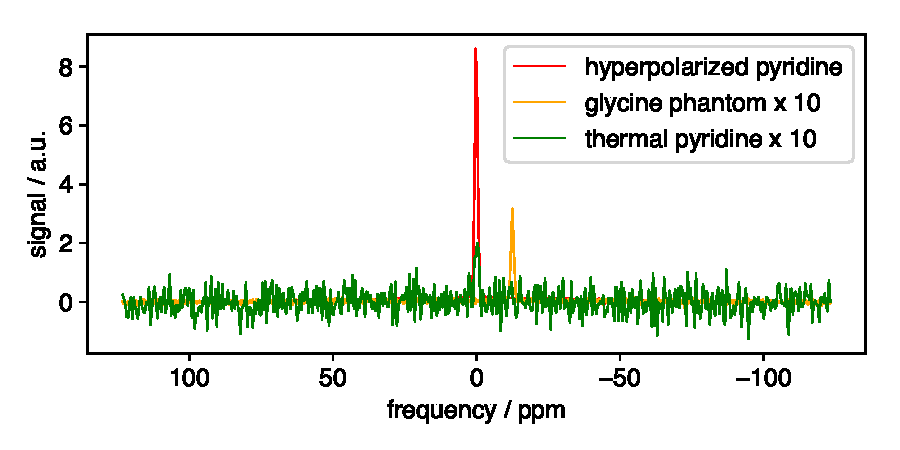
\includegraphics[width=0.99\textwidth]{/figures/experiments/15NSabre/polarization/highPolarization.pdf}
            \caption{15N spectra of the hyperpolarized 15N pyridine sample, the sample in its thermal state and the 15N glycine phantom. Note the frequency shift due to the different chemical shift properties of the two molecules. The relative signal intensity of the hyperpolarized sample is 38.2, additionally, the thermal signal was averaged 250 times. Note the high noise levels on the thermal measurement due to signal averaging.}
        \end{figure}
    \subsection{High field Sabre}
        High field sabre results from the IMTEK \SI{600}{\mega\hertz} spectrometer were obtained. These results show that small amounts of substrate can be hyperpolarized in situ both through the less efficient spontaneous hyperpolarization as well as through pulsed hyperpolarization (Light-Sabre, \todo{ref}).
\section{Simulations}
        \label{sec:results:sim}
        \subsection{Static magnetic field calculations}
        \label{sec:results:sim:B0}
            Using the Biot Savart law, a Matlab program to calculate the fields of current carrying conductors was implemented. Structural elements were mostly solenoids, but also saddle and helmholtz coils were considered.
            \subsubsection{Solenoid Coil}
            The magnetic field of the coil used in the low field NMR system was calculated and the length of the compensation windings was optimized for field homogeniety.
                \begin{figure}
                    \centering
                    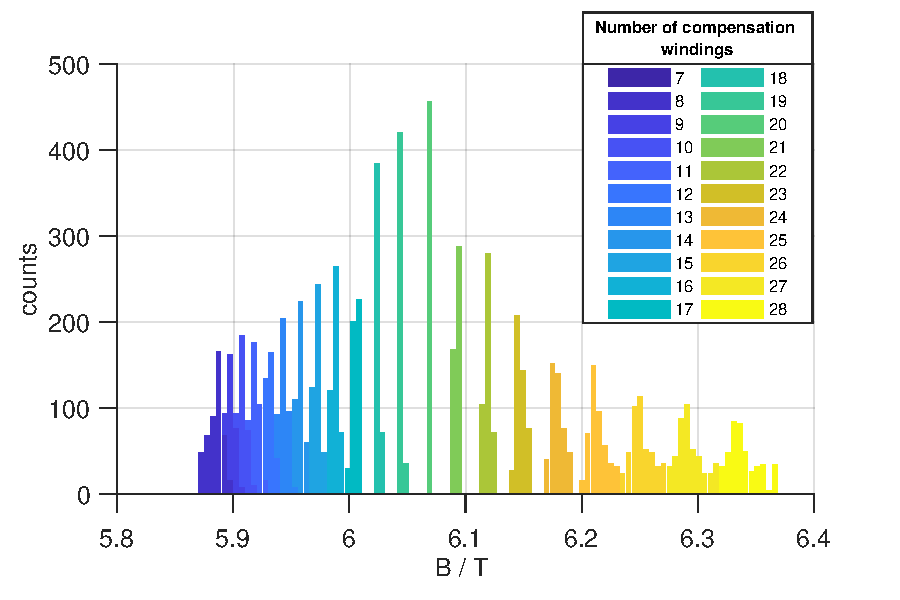
\includegraphics[width=0.99\textwidth]{/figures/simulations/B0/solenoidCoil/compensationWinds.pdf}
                    \caption[Compensation wind optimization]{Histograms of the magnetic field strength. From left to right, number of compensation windings rise. This leads to a field increase and change in homogeniety. Central winding numbers are the most homogenous ones discovered.}
                    \label{fig:results:compensationWindOptimization}
                \end{figure}
            It can be seen that different numbers of turns for the optimization windings change both the overall field strength (simple superposition) as well as its homogeniety. Binning was chosen rough at first to easily discover the overall region of high homogeniety and then refined to streamline in this region.
            The field of the optimized case coil is plotted in figure \todo{ref} both in a plane perpendicular to and parallel to the magnetic fields main direction. Despite the simulations considering to solenoidal character of the coil, rotation of the plane parallel to the magnetic field did not affect homogeniety greatly (\todo{make figs}). The overall shape of the field histogram is not a lorentian; this confirms what was found for rather wide peaks (> \SI{100}{\hertz} linewidth) fitted with lorentians that showed poor resemblance to a lorentian distribution.
        \subsubsection{Helmholtz Array}
        The previously used program was used again to simulate the field of the helmholtz array used in later experients. The simulations were used to optimize the parameters for the setup before manufacture. Simulation steps for the distance between the two helmholtz pairs are shown in figure \ref{fig:results:optimizationSteps}.
        \begin{figure}
            \centering
            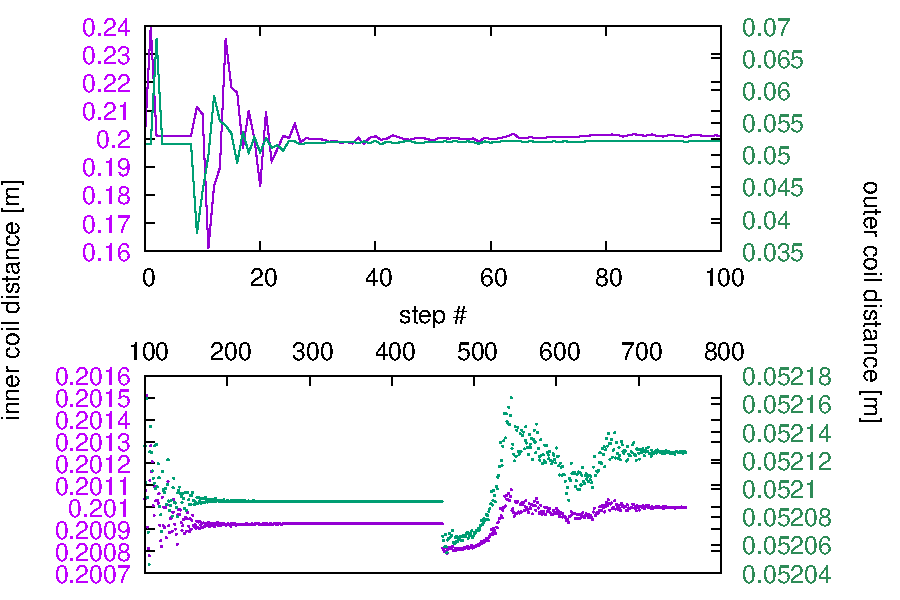
\includegraphics[width=0.99\textwidth]{/figures/simulations/B0/helmholtzCoil/optimizationSteps.pdf}
            \caption[Helmholtz coil optimization]{Optimization steps of the two distances of inner and outer coil pair. Note the small range in the lower graph that is probably already inside the margin of error of manufacture and actual positioning.}
            \label{fig:results:optimizationSteps}
        \end{figure}
        Note that the figures shown here do not include the optimization of the current ratio between the two coil pairs. The simulation results concerning the positions of the coils are shown in figure \ref{fig:results:distanceVariation}. A closeup of the central region is plotted in figure \ref{figure:results:fieldSpread}. The optimal result is marked, and the field homogeniety is plotted for this result (figure \todo{ref, fig}). Comparing the field map to figure \ref{} shows a factor \todo{nn} improvement.
        \begin{figure}
           \centering
           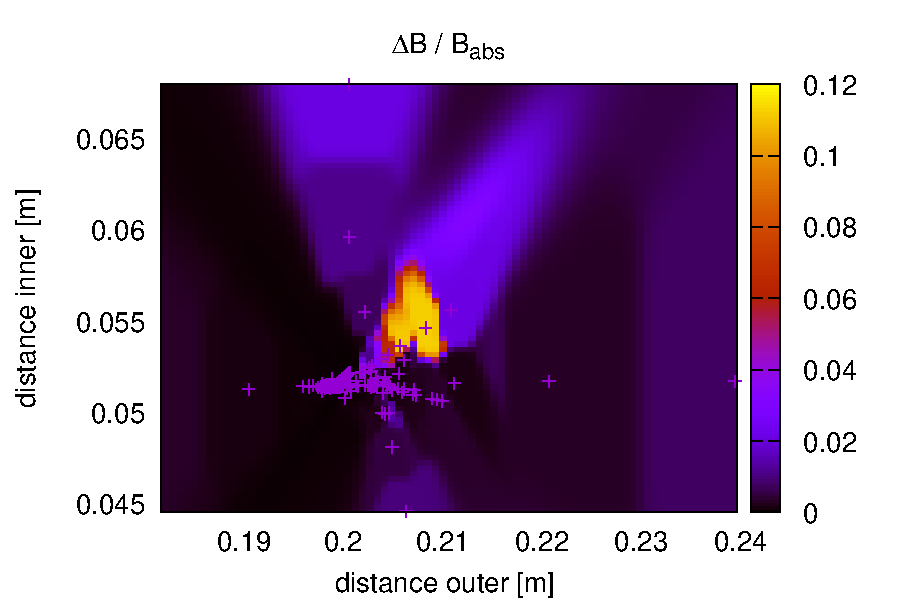
\includegraphics[width = \textwidth]{/figures/simulations/B0/helmholtzCoil/distanceVariation.pdf}
           \label{fig:results:distanceVariation}
           \caption[Optimization steps]{Optimization of the coils distances by 'fminsearchbnd'. Note that the current ratio of the coils was also varied in the simulations, but kept constant for the recording of the data shown here. The value displayed is the ratio of the field spread in the active volume of the coil and the absolute field strength. The black area in the center is where field homogeniety is highest.}
        \end{figure}
        \begin{figure}
            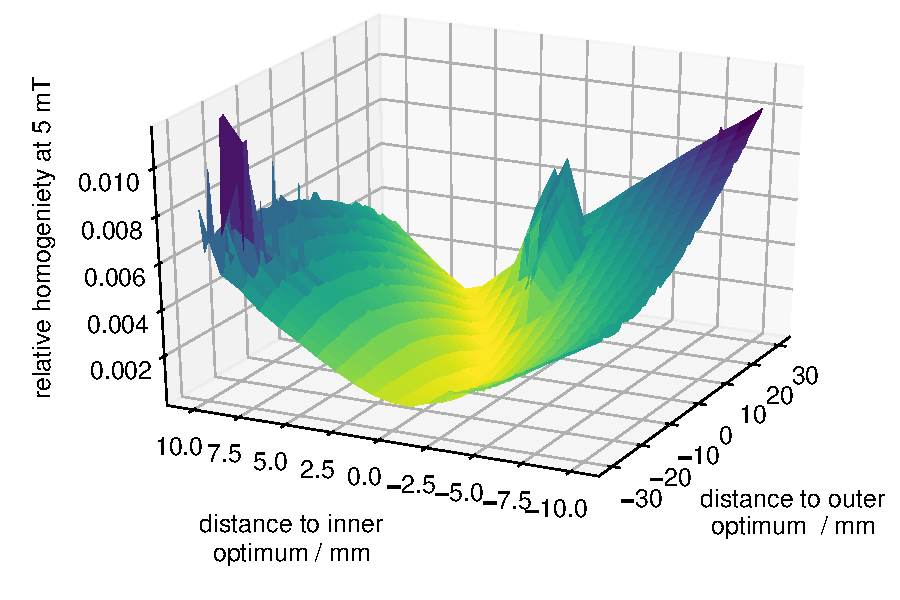
\includegraphics[width = 0.99\textwidth]{/figures/simulations/B0/helmholtzCoil/fieldSpread.pdf}
            \label{fig:results:fieldSpread}
            \caption{3D plot of the central region of high homogeniety shown in \ref{fig:results:distanceVariation}. Note that the distance variation of the inner coil has a more prominent effect on field homogeniety than the outer one. The minimum value found is a relative spread of $5\cdot 10^{-5}$.}
        \end{figure}
        The lowest value found is a relative spread of $4.6 \cdot 10^{-5}$ corresponding to a linewidth of \SI{12.5}{\hertz}. Experimentally, similar values were observed (see chapter \ref{chap:results:lowFieldNMR}). Small variations in the distances lead to strong decrease in homogeniety especially for the inner coil pair - \SI{0.1}{\milli\meter} variations already make up for a decrease of 3 in homogeniety in the inner coil pair while for the outer pair, the same variation makes up for an increase by a factor of 0.2 only. Overall, exact positioning is thus crucial, going especially for the inner pair. The dual helmholtz design has thus increased homogeniety to linewidths smaller than those of the solenoid with compensation windings and linear shims. Adding shims to the helmholtz array is possible and encouraged for future work and will probably further improve homogeniety.
        \subsubsection{Nicotinamide level anti crossings using the spin framework}
        The spin framework developed in this group \todo{ref} was used to calculate level anti crossings for nicotinamide and IR-IMes as a spin system. The results obtained are similar to results previously published concerning pyridine and IR-IMes \todo{ref}. In figure \ref{figure:results:simulation:nicotinamideSpinSystem} the polarization levels are plotted against field and contact time of the complex (i.e. spin evolution time). These results indicate highest polarizations at \SI{4.9}{\milli\tesla} which is close to the fields obtained in the pyridine simulations. A contact time of \SI{10}{\milli\second} seems best to generate high polarizations and needs to be adjusted indirectly via sample temperatures. These results were used to adjust experimental parameters in the best possible way and were confirmed through field and temperature variations (section \ref{chapter:results:lowFieldNMR})
        \begin{figure}
            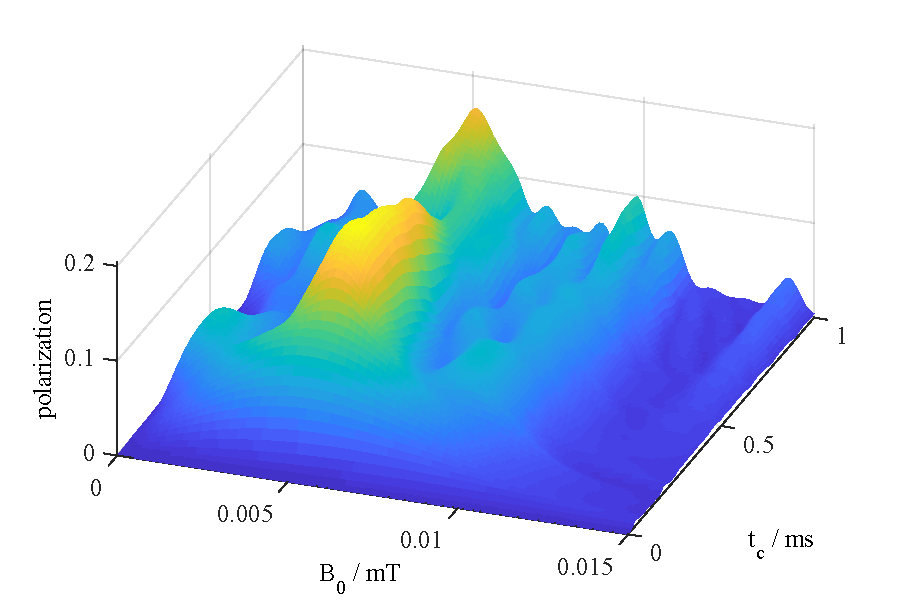
\includegraphics[width=0.99\textwidth]{/figures/simulations/15NSabre/spinFramework/fieldContactTimeDependence.pdf}
            \caption[Spin density matrix calculations]{The }
        \end{figure}
